\section{Задание 1 --- Анализ биоритмов в JavaScript}

Введите дату рождения

\begin{center} 
  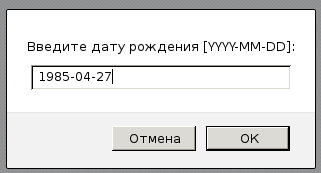
\includegraphics[width=9cm]{img/01.png}
\end{center}

Введите прогнозируемый год

\begin{center} 
  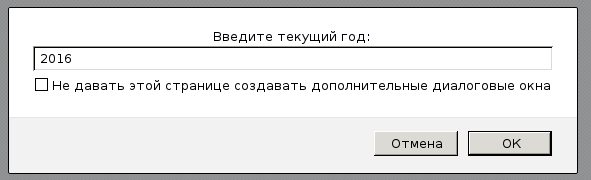
\includegraphics[width=9cm]{img/02.png}
\end{center}

Получившийся график:

\begin{center} 
  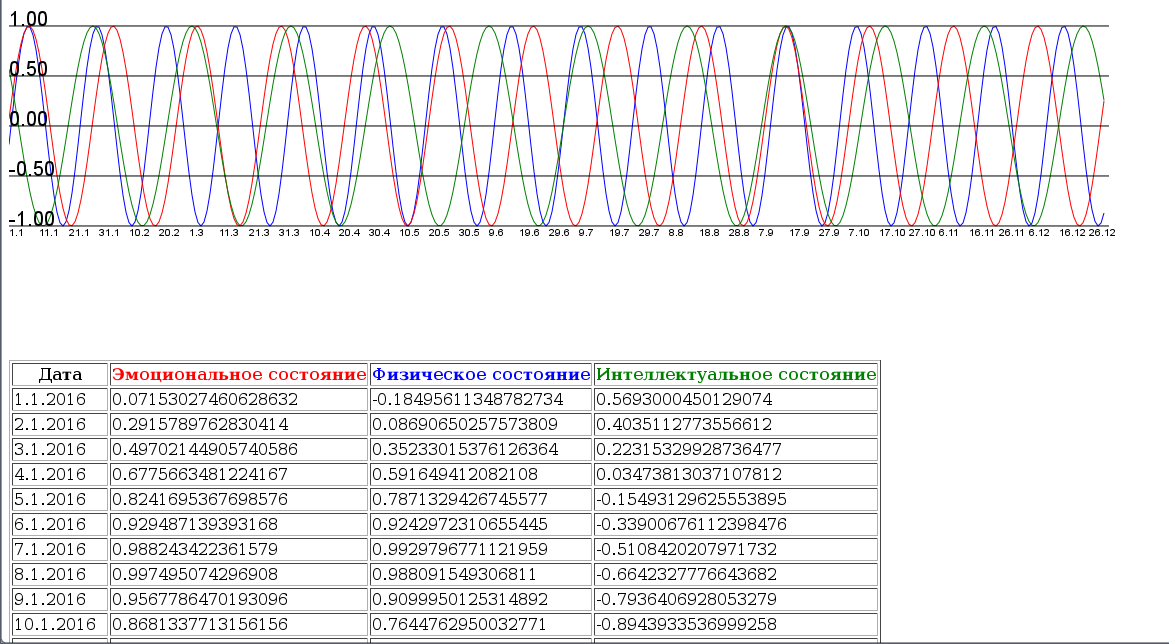
\includegraphics[width=15cm]{img/03.png}
  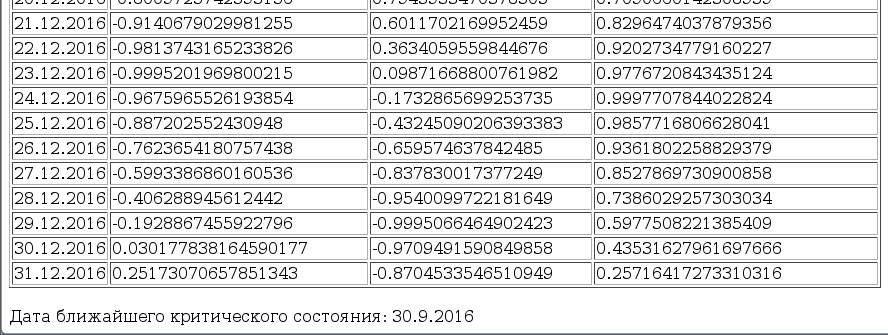
\includegraphics[width=15cm]{img/04.png}
\end{center}

Исходный код \verb|biorhythm.html|:

\begin{verbatim}
<!doctype html>
<html>
  <head>
    <title>Биоритмы</title>
    <meta charset='utf-8' />
  </head>
  <body>
    <canvas id='example'>Обновите браузер</canvas>
    <script>
      var str = prompt("Введите дату рождения [YYYY-MM-DD]:",
                       "1985-04-27");
      var birthDate = new Date(str);
      str = prompt("Введите текущий год: ", "2016");
      var currentYear = new Date(str);
      var changingDate = currentYear;
      var i = currentYear.getFullYear();
      var example=document.getElementById("example"),
          ctx=example.getContext('2d');
      example.height=380; example.width=1200;
      var X=3, YP=0, YPP=0, YE=0, YEP=0, YI=0, YIP=0;
      YPP = Math.sin(2*3.14*(changingDate - birthDate)/
                     (24*60*60*1000*23));
      YEP = Math.sin(2*3.14*(changingDate - birthDate)/
                     (24*60*60*1000*28));
      YIP = Math.sin(2*3.14*(changingDate - birthDate)/
                     (24*60*60*1000*33));
      //Y = -Math.sin(2*3.14*(changingDate - birthDate)/
      //(24*60*60*1000*23))*100+150;
      //ctx.strokeStyle="blue";
      //ctx.moveTo(0,Y);
      ctx.font = "10px Arial";
      var criticalState = YPP+YEP+YIP;
      var criticalMonth = changingDate.getFullYear();
      var criticalDay = changingDate.getDate();
      document.write("<table border=\"1\">");
      document.write(
          "<tr><th>Дата</th><th>" +
              "<font color=\"red\">Эмоциональное с"+
              "остояние</font>" +
              "</th><th><font color=\"blue\">Физи" +
              "ческое состояние</font>" +
              "</th><th><font color=\"green\">Инт" +
              "еллектуальное состояние</font>"+
              "</th></tr>");
      document.write("<tr><td>"+ changingDate.getDate() +
                     "." + (changingDate.getMonth() + 1)+
                     "." + changingDate.getFullYear() +
                     "</td><td>" + YEP +
                     "</td><td>" + YPP +
                     "</td><td>" + YIP +
                     "</td></tr>");
      
      changingDate.setDate(changingDate.getDate()+1);
      while ((changingDate.getFullYear()) == i) {
          YP = Math.sin(2*3.14*(changingDate - birthDate)/
                        (24*60*60*1000*23));
          YE = Math.sin(2*3.14*(changingDate - birthDate)/
                        (24*60*60*1000*28));
          YI = Math.sin(2*3.14*(changingDate - birthDate)/
                        (24*60*60*1000*33));
          
          document.write("<tr><td>"+ changingDate.getDate() +
                         "." + (changingDate.getMonth() + 1)+
                         "." + changingDate.getFullYear() +
                         "</td><td>" + YE +
                         "</td><td>" + YP +
                         "</td><td>" + YI +
                         "</td></tr>");
          
          if (criticalState > (YP+YE+YI)){
              criticalState = YP+YE+YI;
              criticalMonth = changingDate.getMonth();
              criticalDay = changingDate.getDate();
          }
          
          // Строим эмоциональный график
          ctx.beginPath();
          ctx.strokeStyle = "red";
          ctx.moveTo(X-3, 150-YEP*100);
          ctx.lineTo(X, 150-YE*100);
          ctx.stroke();
          
          // Строим физический график
          ctx.beginPath();
          ctx.strokeStyle = "blue";
          ctx.moveTo(X-3, 150-YPP*100);
          ctx.lineTo(X, 150-YP*100);
          ctx.stroke();
          
          // Строим интеллектуальный график
          ctx.beginPath();
          ctx.strokeStyle = "green";
          ctx.moveTo(X-3, 150-YIP*100);
          ctx.lineTo(X, 150-YI*100);
          ctx.stroke();
          
          changingDate.setDate(changingDate.getDate()+1);
          if (X%30 == 0)
              ctx.fillText(changingDate.getDate()+
                           "."+
                           (changingDate.getMonth()+
                            1),X,260);
          X = X+3;
          
          YPP = YP;
          YEP = YE;
          YIP = YI;
      }
      
      document.write("</table>");
      document.write("<br>Дата ближайшего критического состояния: " +
                     criticalDay + "." + (criticalMonth + 1) +
                     "." + i + "<br>");
      
      // Рисуем оси координат
      ctx.beginPath();
      ctx.moveTo(0,150);
      ctx.strokeStyle="black";
      ctx.lineTo(1100,150);
      ctx.font = "20px Arial";
      ctx.fillText("0.00", 0, 150);
      ctx.moveTo(0,50);
      ctx.lineTo(1100,50);
      ctx.fillText("1.00",0,50);
      ctx.moveTo(0,100);
      ctx.lineTo(1100,100);
      ctx.fillText("0.50",0,100);
      ctx.moveTo(0,200);
      ctx.lineTo(1100,200);
      ctx.fillText("-0.50", 0,200);
      ctx.moveTo(0,250);
      ctx.lineTo(1100,250);
      ctx.fillText("-1.00", 0,250);
      ctx.stroke();
    </script>
  </body>
</html>
\end{verbatim}
